\section{Siamese Multi-Object Tracking}
\label{sec:SiamMOT}

This section is dedicated to the most important tracker we have encountered during our research, called \modelname{SiamMOT}~\cite{shuai2021siammot}. Its importance stems from the fact that the majority of our experiments adopted this model. Even though this section could be part of the theoretical foundations chapter, we found it more comprehensible to provide the description of the base architecture closer to the description of our methods and experiments.

\subsection{General Description}

The authors of~\cite{shuai2021siammot} tracker focused on improving online \gls{mot}. As far as their methodology was concerned, they employed region-based approach~\cite{Ren2017} in conjunction with a Siamese multi-object tracking network, hence the name \modelname{SiamMOT}. Broadly speaking, this architecture employes Siamese tracker for motion estimation between two frames. We would like to note that all the principles so far discussed regarding Siamese trackers apply here. However, as already suggested, the adoption of \gls{rpn} enables this framework to have more information available. Not only there is the motion prediction from the Siamese tracker, there are also detections produced by the \modelname{Faster R-CNN} object detector~\cite{Ren2017} that is integrated within the whole architecture. Subsequently, an online solver is utilized to merge these prediction obtained from the tracker and detector heads. It is no surprise that such a framework that exploits modern approaches (more on that later) to object detection and Siamese tracking produces \gls{sota} performance.

We will disect this framewrok in great detail since we studied it scrupulously. We performed multiple experiments, many of which did not yield expected improvements. Nevertheless, the practical part of our work was focused on contributing to the open source repository dedicated to this project developed by several Amazon researchers~\cite{siammotoriggithub}. We followed a standard path of how contributing to open source projects should be done in a transparent and, more importantly, compatible fashion. We initialized a fresh fork of this project on our personal GitHub account~\cite{siammotforkgithub} to preserve as much compatibility with the original software as possible and to not strip ourselves of the opportunity to easily receive potential updates from the original repository.

During our development we often engaged in discussions related to this project incentivized by other researchers who were also working on this project and trying to either only apply this work to their specific use case or even extend the model. Our detailed knowledge of this model acquired through deliberate and long-lasting work on this project often helped several other programmers who dealt with various issues. From the programming standpoint, our work involved a considerable amount of programming, even though the base architecture was provided and fully functional. We would like to emphasize that the project consisted of $?$ lines of source code programmed purely in Python programming language. Concerning the deep learning aspect, the PyTorch library~\cite{NEURIPS2019_9015} was primarily used. It is a widely known library aimed at building deep neural network models while exploiting automatic differentiation.

\subsection{Model Architecture}

\begin{figure}[t]
    \centering
    \includegraphics[width=\linewidth]{figures/methodology/siammot_architecture.pdf}
    \caption[\modelname{SiamMOT} architecture]{The base architecture of the \modelname{SiamMOT} model. This tracker detects and associates object instances simultaneously. The Siamese tracker situated in the top branch serves the purpose of predicting motion of objects across frames, thus faciliates temporal linking of objects in an online fashion. Simply put, the Siamese tracker module can be thought of as a single object tracker with all the pros and cons we have discussed so far. On the other hand, a $2$-stage object detection is performed as part of the bottom branch. These two branches are then merged using a solver that spatially and temporally attemps to match tracker and detector predictions to produce the tracker output. We note that the spatial matching and solver blocks are only used during the inference and are not differentiable. \externalsrc{\cite{shuai2021siammot}}}
    \label{fig:SiamMOTArchitecture}
\end{figure}

\subsection{Training Phase}

\subsection{Inference Phase}

\begin{figure}[t]
    \centering
    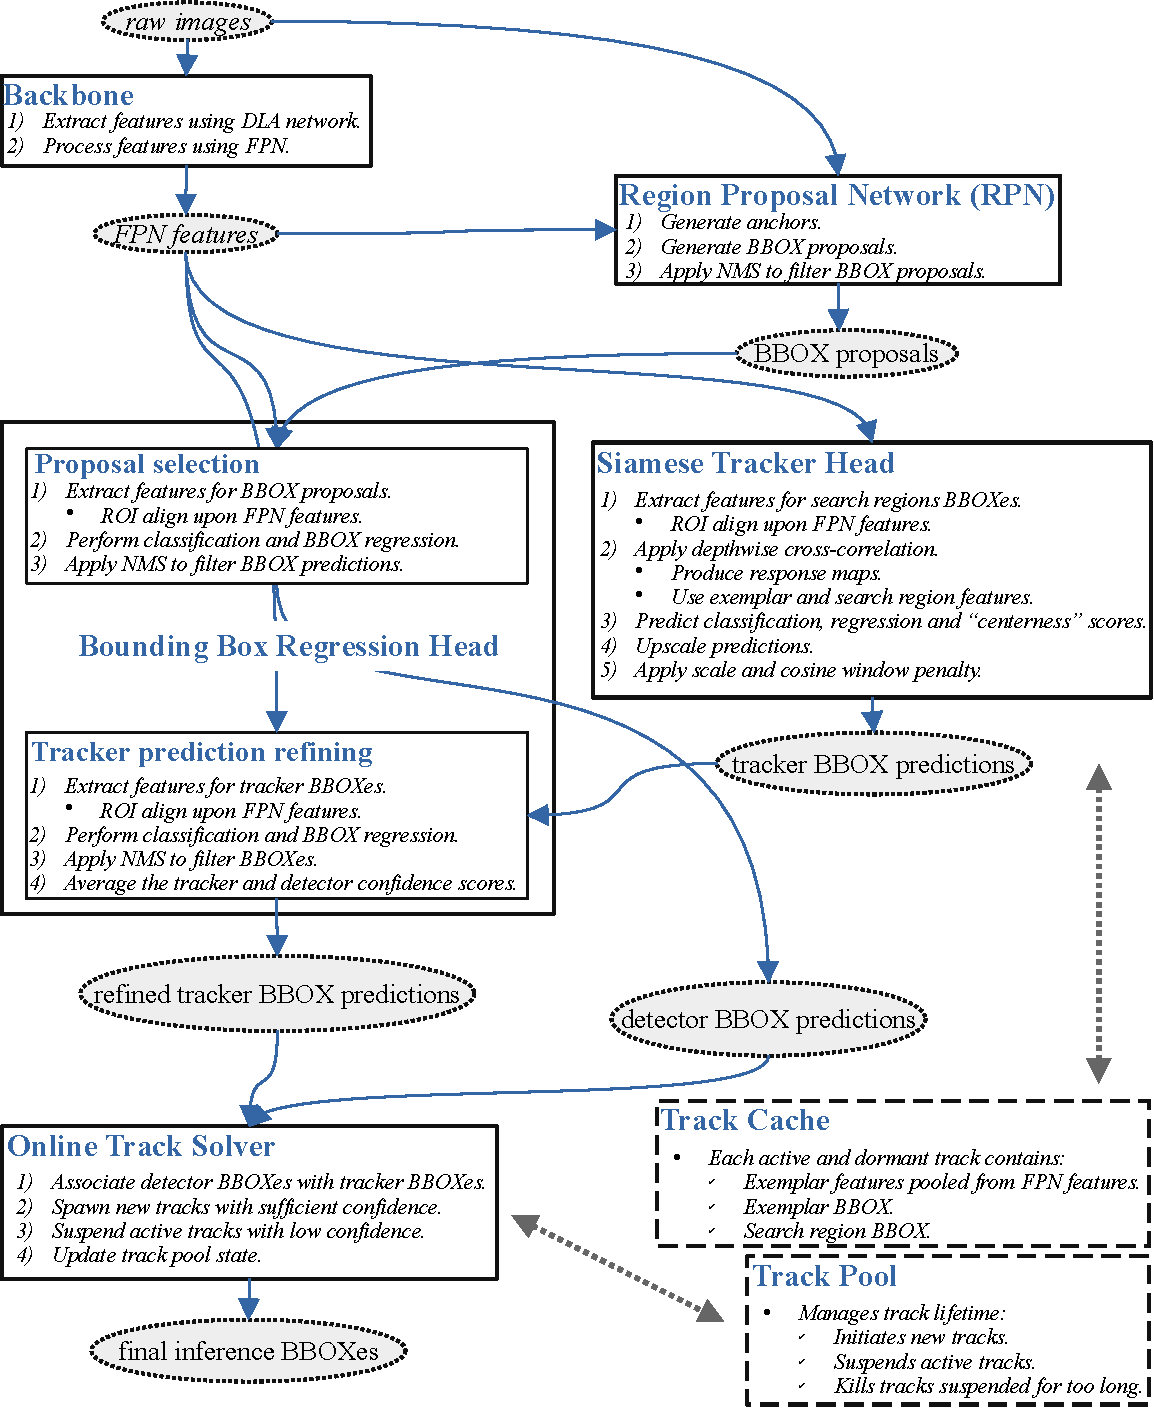
\includegraphics[width=\linewidth]{figures/methodology/siammot_inference_diagram.pdf}
    \caption[\modelname{SiamMOT} inference diagram]{Visualization of the inference pipeline in the \modelname{SiamMOT} architecture. The entire framework efficiently reuses as much information as possible, making it fast and accurate. Backbone features that are a result of intricate \gls{dla} and \gls{fpn} processing are fed into detector and the tracker. Please note that the predictions from the tracker are once again refined using the detector head. Two two aforementioned heads function on top of backbone features through the lens of \gls{roi} align operations. During the inference phase, the ``online solver'' works only with the final \glspl{bbox} produced by the tracker and the object detector. It utilizes a simple caching mechanism to store the backbone features belonging to active or dormant objects. The decision making regarding initialization, suspension and complete removal of track is performed within the ``track pool'' module.}
    \label{fig:SiamMOTInference}
\end{figure}

\subsection{Implementation Details}

\subsection{Experimental Analysis}
